% Parte 2: resultados, conclusiones y limitaciones.
% Se incluye desde informe.tex; no compilar este archivo solo.

% ===========================================================================
\section{Resultados y visualizaciones}
% ===========================================================================

\subsection{Escenario 1: paracaidista}

El Cuadro~\ref{tab:paracaidista-res} resume las métricas de cada modelo y la Figura~\ref{fig:paracaidista} muestra la evolución de la altura, la rapidez y la aceleración. $t_{95}$ es el tiempo necesario para alcanzar el \qty{95}{\percent} de la velocidad terminal y $d_{95}$ la distancia recorrida hasta ese instante.

\begin{table}[H]
  \centering
  \small
  \caption{Resultados del paracaidista (RK4, $\Delta t = \qty{0.01}{s}$).}
  \label{tab:paracaidista-res}
  \begin{tabular}{@{}lrrrrr@{}}
    \toprule
    Modelo & \thead{$\vt$\\(m/s)} & \thead{$t_{95}$\\(s)} & \thead{$d_{95}$\\(m)} & \thead{Tiempo de\\caída (s)} & \thead{Rapidez de\\impacto (m/s)} \\
    \midrule
    Vacío      & ---    & ---    & ---   & 28.557 & 280.143 \\
    Lineal     & 50.622 & 15.459 & 534.4 & 84.177 & 50.622 \\
    Cuadrático & 50.622 & 9.452  & 304.1 & 82.593 & 50.622 \\
    \bottomrule
  \end{tabular}
\end{table}

\begin{figure}[H]
  \centering
  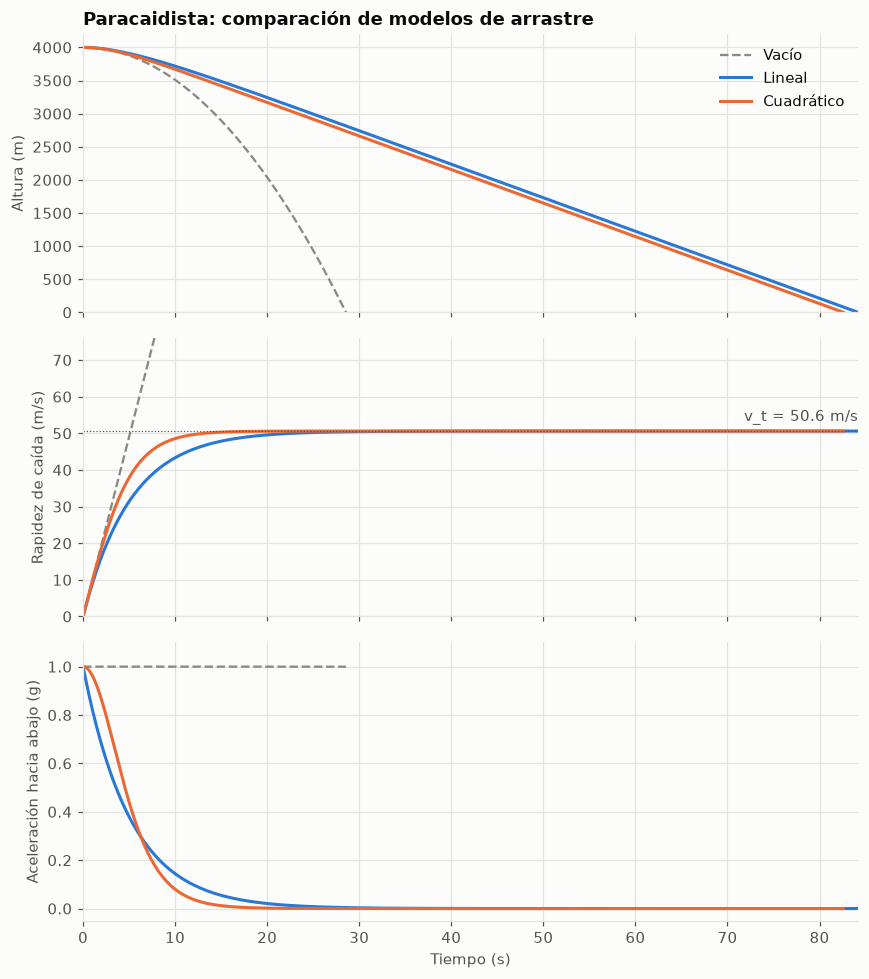
\includegraphics[width=0.82\textwidth]{paracaidista_modelos.png}
  \caption{Paracaidista: altura, rapidez de caída $\lvert v\rvert$ y aceleración hacia abajo (en unidades de $g$) para los tres modelos. En la aceleración, 1 corresponde a caída libre sin aire y 0 al régimen terminal. La línea punteada horizontal marca $\vt = \qty{50.6}{m/s}$.}
  \label{fig:paracaidista}
\end{figure}

\paragraph{Validación.} Los valores simulados coinciden con las fórmulas de la Sección~\ref{sec:analiticas}:
\begin{itemize}
  \item Vacío: $\sqrt{2\cdot 4000/9.81} = \qty{28.5569}{s}$ y $\sqrt{2\cdot 9.81\cdot 4000} = \qty{280.143}{m/s}$. Simulado: \qty{28.5569}{s} y \qty{280.143}{m/s}.
  \item Lineal: $t_{95} = 5.160\ln 20 = \qty{15.459}{s}$. Simulado: \qty{15.459}{s}.
  \item Cuadrático: $t_{95} = 5.160\,\atanh(0.95) = \qty{9.452}{s}$ y $t_{\text{imp}} = \qty{82.5935}{s}$. Simulado: \qty{9.452}{s} y \qty{82.5935}{s}.
\end{itemize}

\paragraph{Discusión.}
Aunque ambos modelos tienen la misma velocidad terminal, el cuadrático llega al \qty{95}{\percent} de $\vt$ en \qty{9.5}{s} y el lineal en \qty{15.5}{s}, es decir, un \qty{64}{\percent} más tarde. La razón está en la forma de cada ley: el arrastre cuadrático es débil a baja rapidez, por lo que al principio el cuerpo acelera casi como en el vacío, pero crece muy rápido al acercarse a $\vt$, lo que produce una transición más abrupta. El arrastre lineal, en cambio, frena desde el primer instante y se aproxima a $\vt$ más lentamente. Esto se observa con claridad en el panel inferior de la Figura~\ref{fig:paracaidista}: la aceleración del modelo lineal disminuye de inmediato, mientras que la del cuadrático se mantiene cerca de $1\,g$ durante los primeros segundos y luego cae bruscamente.

Como el paracaidista pasa unos \qty{70}{s} en régimen terminal, los tiempos totales de caída de ambos modelos difieren solo en \qty{1.6}{s} (\qty{2}{\percent}); la diferencia entre modelos se concentra en los primeros 15 a \qty{20}{s}. En régimen terminal el paracaidista desciende unos \qty{50}{m} cada segundo, por eso la curva de altura es casi una recta durante la mayor parte del salto.

Sin aire, el paracaidista llegaría al suelo en \qty{28.6}{s} a \qty{280}{m/s} (\qty{1008}{km/h}), una rapidez 5.5 veces mayor que con aire. La resistencia del aire, por tanto, no es un detalle en este problema: determina por completo el resultado.

\subsection{Escenario 2: pelotas}

El Cuadro~\ref{tab:pelotas-res} resume los resultados de la caída de las cuatro pelotas. La Figura~\ref{fig:pelotas-tray} muestra las trayectorias y la Figura~\ref{fig:pelotas-resumen} condensa el escenario en dos indicadores.

\begin{table}[H]
  \centering
  \small
  \caption{Resultados de las pelotas desde \qty{56}{m} (RK4, $\Delta t = \qty{0.01}{s}$).}
  \label{tab:pelotas-res}
  \begin{tabular}{@{}lrrrrrr@{}}
    \toprule
    Pelota & \thead{$\vt$\\(m/s)} & \thead{Tiempo de\\caída (s)} & \thead{Retraso vs.\\vacío (s)} & \thead{Rapidez de\\impacto (m/s)} & \thead{\% de $\vt$\\al impactar} & \thead{$Re$ al\\impactar} \\
    \midrule
    Ping-pong & 8.557  & 7.149 & 3.770 & 8.557  & 100.0 & \num{23165} \\
    Tenis     & 23.677 & 3.948 & 0.569 & 21.946 & 92.7  & \num{99515} \\
    Béisbol   & 34.266 & 3.647 & 0.269 & 26.712 & 78.0  & \num{132336} \\
    Boliche   & 82.168 & 3.425 & 0.046 & 31.843 & 38.8  & \num{465506} \\
    Vacío     & ---    & 3.379 & 0     & 33.147 & ---   & --- \\
    \bottomrule
  \end{tabular}
\end{table}

\paragraph{Validación.} En el vacío, $\sqrt{2\cdot 56/9.81} = \qty{3.3789}{s}$ y $\sqrt{2\cdot 9.81\cdot 56} = \qty{33.147}{m/s}$. Simulado: \qty{3.3789}{s} y \qty{33.147}{m/s}.

\begin{figure}[H]
  \centering
  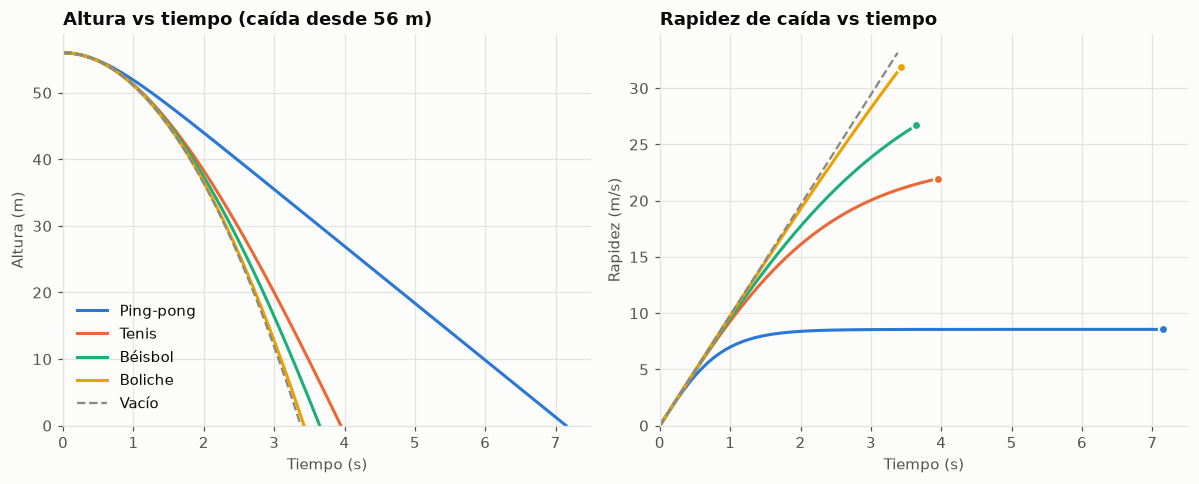
\includegraphics[width=\textwidth]{pelotas_trayectorias.png}
  \caption{Altura y rapidez de caída contra el tiempo para las cuatro pelotas y la caída en el vacío. El punto al final de cada curva de rapidez marca el impacto con el suelo.}
  \label{fig:pelotas-tray}
\end{figure}

\begin{figure}[H]
  \centering
  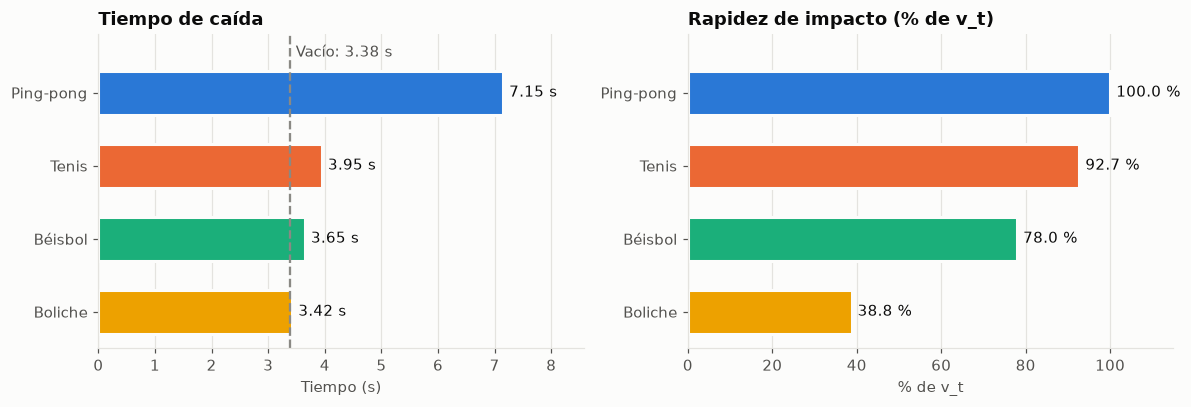
\includegraphics[width=\textwidth]{pelotas_resumen.png}
  \caption{Izquierda: tiempo de caída de cada pelota; la línea discontinua indica el tiempo en el vacío. Derecha: rapidez de impacto como porcentaje de la velocidad terminal de cada pelota.}
  \label{fig:pelotas-resumen}
\end{figure}

\paragraph{Discusión.}
Lo que determina la influencia del aire no es la masa por sí sola, sino la relación $m/k$, es decir, la masa frente al área. Como $\vt = \sqrt{mg/k}$, una pelota pesada y compacta tiene una velocidad terminal alta y en una caída de \qty{56}{m} apenas nota el aire.

\begin{itemize}
  \item La bola de boliche llega solo \qty{0.046}{s} después que en el vacío (\qty{1.4}{\percent} más tarde). A simple vista caería ``como en el vacío'', lo que es coherente con la observación atribuida a Galileo. Al impactar apenas ha alcanzado el \qty{38.8}{\percent} de su velocidad terminal.
  \item La pelota de ping-pong alcanza su velocidad terminal (\qty{8.56}{m/s}) en menos de \qty{2}{s} y recorre el resto de la altura a rapidez constante: tarda \qty{7.15}{s}, más del doble que en el vacío.
  \item Las pelotas de tenis y de béisbol son casos intermedios: se separan claramente de la curva del vacío en la segunda mitad de la caída.
\end{itemize}

En cuanto al experimento de Galileo, en el vacío las cuatro pelotas caen exactamente igual. Con aire, la bola de boliche y la pelota de béisbol llegan al suelo con \qty{0.22}{s} de diferencia; cuando la bola de boliche toca el suelo, la de béisbol todavía está a unos \qty{6}{m} de altura.

Todos los números de Reynolds son mucho mayores que 1, lo que justifica el uso del modelo cuadrático. Las pelotas de ping-pong, tenis y béisbol ($Re$ entre \num{2e4} y \num{1.3e5}) están en el rango en que el $C_d$ de una esfera es aproximadamente constante. La bola de boliche ($Re \approx \num{4.7e5}$) ya se encuentra en la zona de la \emph{crisis de arrastre}, que para esferas lisas comienza alrededor de $Re \approx \num{2e5}$ a \num{3e5} y en la que $C_d$ puede disminuir bruscamente~\cite{white}. Sin embargo, como el aire solo modifica su tiempo de caída en un \qty{1.4}{\percent}, esto no altera las conclusiones.

\subsection{Escenario 3: convergencia y comparación de métodos}

\subsubsection{Orden de convergencia observado}

La Figura~\ref{fig:convergencia} muestra el error máximo contra el paso de tiempo en escala log-log y el Cuadro~\ref{tab:ordenes} los órdenes obtenidos con el ajuste descrito en la Sección~\ref{sec:diseno-convergencia}. Los órdenes medidos coinciden con los teóricos con un margen de \qty{1}{\percent}, lo que valida que ambos métodos están correctamente implementados. Las tablas completas de errores, con el orden local entre pasos consecutivos, se encuentran en el Apéndice~\ref{app:tablas}.

\begin{table}[H]
  \centering
  \caption{Orden de convergencia teórico y observado.}
  \label{tab:ordenes}
  \begin{tabular}{@{}llccc@{}}
    \toprule
    Modelo & Método & \thead{Orden\\teórico} & \thead{Orden observado\\en $y$} & \thead{Orden observado\\en $v$} \\
    \midrule
    Lineal     & Euler & 1 & 1.003 & 1.003 \\
    Lineal     & RK4   & 4 & 4.031 & 4.031 \\
    Cuadrático & Euler & 1 & 1.004 & 1.003 \\
    Cuadrático & RK4   & 4 & 3.996 & 4.037 \\
    \bottomrule
  \end{tabular}
\end{table}

\begin{figure}[H]
  \centering
  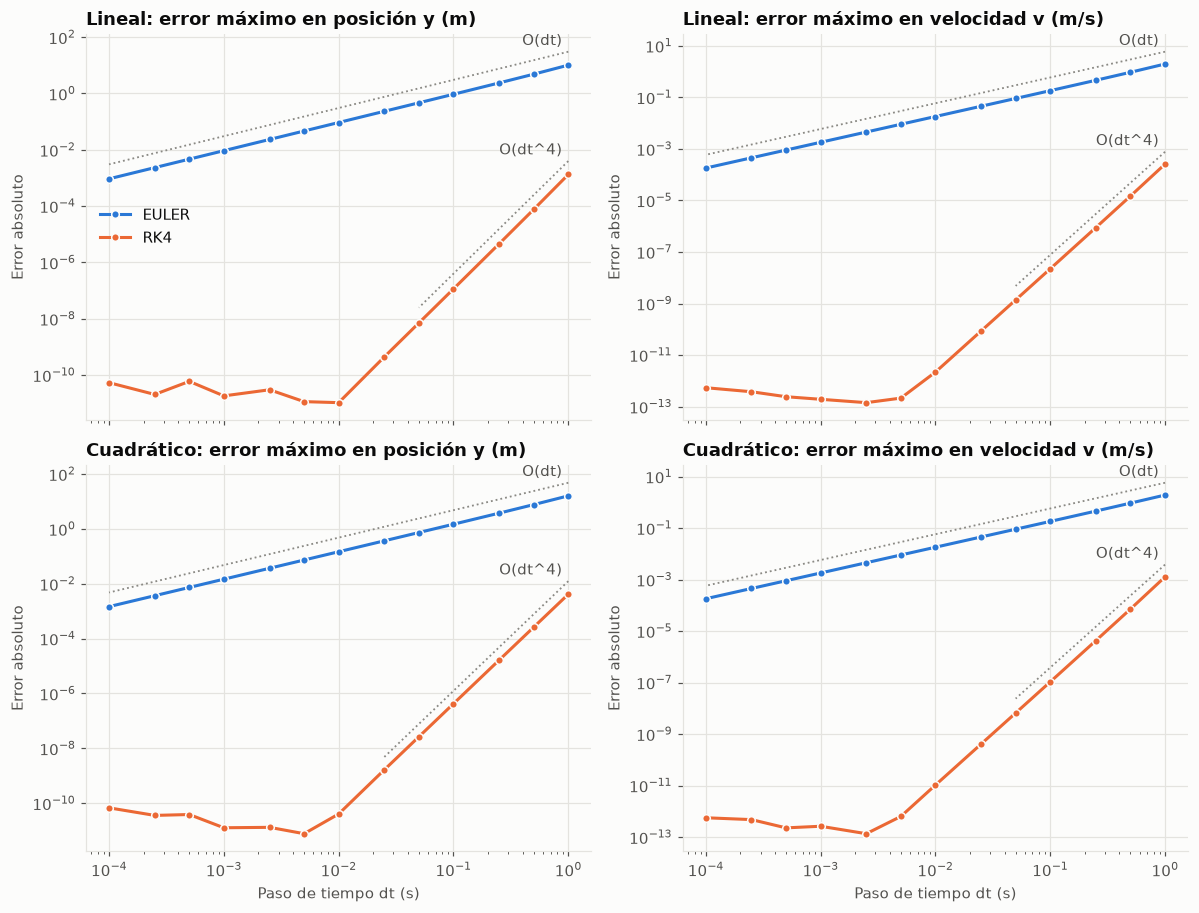
\includegraphics[width=\textwidth]{convergencia.png}
  \caption{Error absoluto máximo en $y$ y en $v$ contra el paso de tiempo $\Delta t$, para los modelos lineal y cuadrático en el intervalo $[0, 20]$~s. Las rectas punteadas son referencias de pendiente 1 y 4.}
  \label{fig:convergencia}
\end{figure}

\subsubsection{Errores y piso de redondeo}

El Cuadro~\ref{tab:errores} muestra una selección de los errores máximos para el modelo cuadrático.

\begin{table}[H]
  \centering
  \caption{Errores máximos seleccionados (modelo cuadrático, intervalo de \qty{20}{s}).}
  \label{tab:errores}
  \begin{tabular}{@{}lllll@{}}
    \toprule
    & \multicolumn{2}{c}{Euler} & \multicolumn{2}{c}{RK4} \\
    \cmidrule(lr){2-3} \cmidrule(l){4-5}
    $\Delta t$ (s) & Error en $y$ (m) & Error en $v$ (m/s) & Error en $y$ (m) & Error en $v$ (m/s) \\
    \midrule
    1      & 16.0   & 1.92    & \num{4.2e-3}  & \num{1.3e-3} \\
    0.1    & 1.48   & 0.182   & \num{4.2e-7}  & \num{1.1e-7} \\
    0.01   & 0.147  & 0.0181  & \num{4.0e-11} & \num{1.0e-11} \\
    0.001  & 0.0147 & 0.0018  & \num{1.3e-11} & \num{2.6e-13} \\
    0.0001 & 0.0015 & 0.00018 & \num{6.8e-11} & \num{5.6e-13} \\
    \bottomrule
  \end{tabular}
\end{table}

De estos resultados se destacan tres observaciones:
\begin{itemize}
  \item RK4 con $\Delta t = \qty{1}{s}$ es más preciso que Euler con $\Delta t = \qty{0.0001}{s}$, aun cuando este último realiza \num{10000} veces más pasos.
  \item \textbf{Piso de redondeo.} Por debajo de $\Delta t \approx \qty{0.01}{s}$ el error de RK4 deja de disminuir y se estanca entre $10^{-13}$ y $10^{-10}$; incluso aumenta ligeramente. En ese punto el error del método ya es menor que el error de redondeo de la aritmética de doble precisión (unos 16 dígitos significativos), que se acumula con el número de pasos. Reducir más el paso no mejora el resultado y solo aumenta el costo de cómputo.
  \item El error de Euler disminuye linealmente en todo el rango estudiado, porque en ningún momento llega al piso de redondeo.
\end{itemize}

\subsubsection{Efecto del método en los escenarios}

El Cuadro~\ref{tab:metodo-escenarios} compara los tiempos de caída obtenidos con cada método usando el paso por defecto. Con $\Delta t = \qty{0.01}{s}$, Euler ya produce resultados útiles, con errores del orden de milisegundos, mientras que RK4 coincide con la solución exacta en todos los dígitos mostrados.

\begin{table}[H]
  \centering
  \caption{Tiempo de caída con Euler y con RK4 ($\Delta t = \qty{0.01}{s}$).}
  \label{tab:metodo-escenarios}
  \begin{tabular}{@{}lrrr@{}}
    \toprule
    Caso & \thead{Euler\\(s)} & \thead{RK4\\(s)} & \thead{Diferencia\\(s)} \\
    \midrule
    Paracaidista, vacío      & 28.5619 & 28.5569 & 0.005 \\
    Paracaidista, cuadrático & 82.5954 & 82.5935 & 0.002 \\
    Ping-pong                & 7.1511  & 7.1491  & 0.002 \\
    Boliche                  & 3.4296  & 3.4249  & 0.005 \\
    Pelotas, vacío           & 3.3839  & 3.3789  & 0.005 \\
    \bottomrule
  \end{tabular}
\end{table}

\subsubsection{Paso de tiempo grande}

Para hacer visible la diferencia entre los métodos se integró el modelo cuadrático del paracaidista con $\Delta t = \qty{2}{s}$ (Figura~\ref{fig:dt-grande}). Euler llega a equivocarse en \qty{4.2}{m/s} a los \qty{6}{s}, en plena transición hacia $\vt$, y sobreestima la rapidez: al usar la aceleración del inicio de cada paso durante todo el paso, ``cree'' que el cuerpo acelera más de lo que realmente lo hace. RK4, con el mismo paso, tiene un error máximo de \qty{0.025}{m/s}, unas 170 veces menor.

En ambos métodos el error disminuye una vez alcanzada la velocidad terminal. Esto se debe a que $\vt$ es un punto de equilibrio estable de la ecuación para $v$: los errores cometidos en pasos anteriores se amortiguan en lugar de acumularse.

\begin{figure}[H]
  \centering
  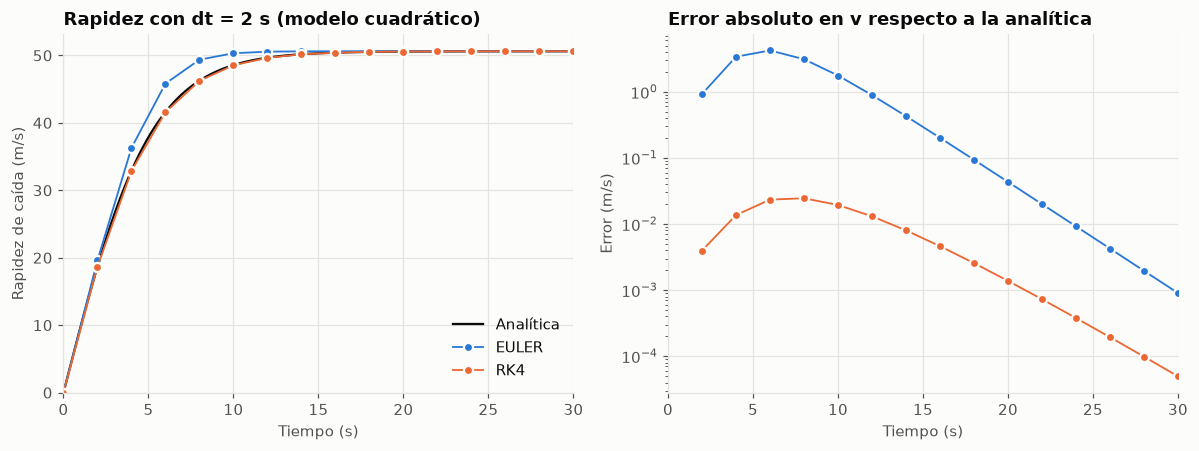
\includegraphics[width=\textwidth]{metodos_dt_grande.png}
  \caption{Izquierda: rapidez de caída del paracaidista (modelo cuadrático) con $\Delta t = \qty{2}{s}$ según la solución analítica, Euler y RK4. Derecha: error absoluto en $v$ respecto a la solución analítica, en escala logarítmica.}
  \label{fig:dt-grande}
\end{figure}

% ===========================================================================
\section{Conclusiones}
% ===========================================================================

\begin{enumerate}
  \item La resistencia del aire cambia cualitativamente la caída: en lugar de acelerar sin límite, el cuerpo tiende a una velocidad terminal $\vt$. Para el paracaidista, esto reduce la rapidez de impacto de \qty{280}{m/s} a \qty{51}{m/s}.
  \item La forma de la ley de arrastre importa aunque la velocidad terminal sea la misma: el modelo cuadrático alcanza el régimen terminal un \qty{39}{\percent} antes que el lineal (\qty{9.5}{s} contra \qty{15.5}{s}).
  \item Para objetos macroscópicos en aire el modelo adecuado es el cuadrático: en todos los casos estudiados $Re$ está entre $10^4$ y $10^7$. El modelo lineal solo es aplicable a partículas microscópicas.
  \item La influencia del aire depende de la relación entre masa y área ($\vt = \sqrt{mg/k}$), no de la masa sola. En \qty{56}{m}, la bola de boliche se comporta casi como en el vacío (\qty{1.4}{\percent} de retraso), mientras que la de ping-pong tarda más del doble.
  \item Euler y RK4 convergen con sus órdenes teóricos (1 y 4; medidos 1.00 y 4.0). RK4 es la mejor opción para este problema: con $\Delta t = \qty{0.01}{s}$ prácticamente alcanza el límite de precisión de la máquina, mientras que Euler necesitaría pasos impracticablemente pequeños para igualarlo.
  \item Reducir el paso de tiempo no siempre mejora el resultado: por debajo de cierto valor domina el error de redondeo.
\end{enumerate}

% ===========================================================================
\section{Limitaciones y sugerencias de trabajo futuro}
% ===========================================================================

El modelo utilizado hace varias simplificaciones que abren posibles extensiones:
\begin{itemize}
  \item \textbf{Densidad del aire constante.} A \qty{4000}{m} la densidad del aire es cerca de un \qty{30}{\percent} menor que a nivel del mar, por lo que la velocidad terminal real al inicio del salto es mayor. Una extensión natural es usar una atmósfera exponencial o el modelo de atmósfera estándar internacional (ISA) para obtener $\rho(y)$. Esto es imprescindible para saltos estratosféricos, como el de Felix Baumgartner en 2012, que superó la velocidad del sonido.
  \item \textbf{Coeficiente de arrastre constante.} En realidad $C_d$ depende de $Re$ (por ejemplo, la crisis de arrastre en esferas) y de la postura del paracaidista. Se podría usar una correlación empírica $C_d(Re)$.
  \item \textbf{Sin apertura del paracaídas.} Se podría cambiar $C_d A$ al alcanzar una altura dada y estudiar la transición entre dos velocidades terminales.
  \item \textbf{Movimiento solo vertical.} Una extensión a dos dimensiones (salto desde un avión en movimiento o con viento lateral) mostraría cómo el arrastre acopla las componentes horizontal y vertical.
  \item \textbf{Sin viento ni efectos de rotación}, como el efecto Magnus en pelotas que giran.
  \item \textbf{Métodos de paso fijo.} Se podría implementar un método adaptativo (por ejemplo, RK45) y una detección de eventos más precisa que la interpolación lineal.
\end{itemize}
